%%%%%%%%%%%%%%%%%%%%%%%%%%%%%%%%%%%%%%%%%%%%%%%%%%%%%%%%%%%%%%%
% 音講論用スタイルファイル onkoron.sty の使用例
%
% 作成:2005年 4月 9日 (初版)
%              4月15日 (Ver.1)
%              4月27日 (Ver.1.1)
%             11月30日 (Ver.1.2)
%       2013年 6月11日 (Ver.1.3)
%
%%%%%%%%%%%%%%%%%%%%%%%%%%%%%%%%%%%%%%%%%%%%%%%%%%%%%%%%%%%%%%%
%\documentclass[11pt,twocolumn]{jarticle} % 11pt(標準)
\documentclass[10pt,twocolumn,uplatex,dvipdfmx]{jsarticle} % 10pt(オプション)
\usepackage{onkoron}
\usepackage{amsmath}
\usepackage{graphicx}
\usepackage{float}
\usepackage{subfig}
\usepackage{url}
\usepackage[ipaex]{pxchfon}
%%%%%%%%%%%%%%%%%%%%%%%%%%%%%%%%%%%%%%%%%%%%%%%%%%%%%%%%%%%%%%%
% 参考文献の引用が [3,6,2,1] -> [1-3,6] になります.
% citesort.sty は,2005年4月現在,下記からダウンロード可能です.
% http://www.utexas.edu/ogs/etd/LaTeX/Style.files/citesort.sty
%
%\usepackage{citesort}

%%%%%%%%%%%%%%%%%%%%%%%%%%%%%%%%%%%%%%%%%%%%%%%%%%%%%%%%%%%%%%%

\setlength\floatsep{0truemm} %set space size between figure and figure
% 行間を標準よりも広くしたい場合には,ここの数字を大きくして
% ください.逆に狭くしたい場合には,数字を小さくしてください.
\renewcommand{\baselinestretch}{1.0}

\makeatletter
\if@twocolumn
  \renewcommand{\paragraph}{\@startsection{paragraph}{4}{\z@}%
    {\z@}{-1zw}% 改行せず 1zw のアキ
    {\normalfont\normalsize\headfont}}
\else
  \renewcommand{\paragraph}{\@startsection{paragraph}{4}{\z@}%
    {0.5\Cvs \@plus.5\Cdp \@minus.2\Cdp}%
    {-1zw}% 改行せず 1zw のアキ
    {\normalfont\normalsize\headfont}}
\fi
\makeatother

%%%%%%%%%%%%%%%%%%%%%%%%%%%%%%%%%%%%%%%%%%%%%%%%%%%%%%%%%%%%%%%
% 論文タイトルおよび脚注用の英文を記載する.
%
\title{交通音の危険性の知覚における老人性難聴の影響\\ : 模擬難聴システムによる検討
\thanks{Effects of age-related hearing loss on perception of traffic risk for approaching car sound : Investigation using hearing impairment simulator.
by FURUYA, Koki, WATANABE, Yuya, and MATSUI, Toshie  (Toyohashi University of Technology)}
}
%%%%%%%%%%%%%%%%%%%%%%%%%%%%%%%%%%%%%%%%%%%%%%%%%%%%%%%%%%%%%%%
% 講演者には○を付す.
% 講演者が粟屋潔学術奨励賞受賞対象者の場合には◎を付す.
%
\author{◎古屋孝基, 渡邊優也, 松井淑恵 (豊橋技科大院)}
%
\begin{document}
\maketitle

%--------------------------------------
\section{はじめに}
%--------------------------------------
高度高齢化社会となりつつある日本では, 老人性難聴の増加が予想されている. 老人性難聴者は音に対する知覚が健聴者と大きく異なる場合があり, 社会の音環境を考えるうえで老人性難聴による聞こえを評価することは非常に重要である.
%の変化は無視できない.
% しかし, 高齢者は認知機能の低下など様々な問題を持つため, 統制のとれたデータ収集が困難である. そのような状況の中, 入野らが健聴者に難聴者の聞こえを呈示できる模擬難聴システムを開発した\cite{nagae2014hearing}.
老人性難聴について統制のとれたデータを収集することは困難であるが, 入野らが開発した模擬難聴システムを用いることで健聴者が難聴者の聞こえを評価でき, 聴覚系の影響のみを調査できるようになった\cite{nagae2014hearing}.
本研究では, 生活の安全性にもっとも関わりの深い音である交通音を聞いたとき, その危険性の評価が老人性難聴の有無によってどのように異なるか調査した. 加えて, 交通事故に大きく関与すると思われる車の走行速度についても老人性難聴による知覚の変化が生じるか検討した.
%\cite{永江美沙貴2014模擬難聴実現のための逆圧縮特性処理とユーザインタフェース}

%--------------------------------------
\section{実験内容}
%--------------------------------------

%-----------------------------------------------------------------
\subsection{模擬難聴システムと圧縮特性}
%-----------------------------------------------------------------

% 健聴者の場合, 入力レベルが30 dB下回る場合や80 dBを上回る場合は蝸牛の入力レベルと蝸牛の内部出力レベルはほぼ比例する. 一方で, 入力レベルが30 dB$\sim$80 dBの間で変化するとき, 入力増加の割合に対して出力増加の割合が小さく, その傾きは圧縮的である. この現象は圧縮特性と呼ばれ, ダイナミックレンジの大きい外界の音を比較的狭い可聴範囲の振動へと変換する役割を担っていると考えられている. 模擬難聴システムでは音に対して逆圧縮特性を付与することで, 健聴者の圧縮特性を打ち消し, 老人性難聴の聞こえを模擬している.
健聴者の場合, 入力レベルが30~dBから80~dBの間で変化するとき, 入力増加の割合に対して出力増加の割合が小さくなる. この現象は圧縮特性と呼ばれ, この機能が低下することが老人性難聴の原因の一つとされる. 模擬難聴システムでは音に対して逆圧縮特性を付与することで, 健聴者の圧縮特性を打ち消し, 老人性難聴の聞こえを模擬できる.

%-----------------------------------------------------------------
\subsection{交通音の危険度評価実験}\label{danger_Exp}
%-----------------------------------------------------------------

% 実験参加者は21歳から22歳の男性10名である. 全員が事前に聴力検査を実施し, 全ての周波数(125-8000Hz)の聴力レベルが20 dBを超えないことを確認した. 実験参加者はヘッドホンから刺激音を聞いてGUI上で回答した. 呈示した刺激音は, 日本建築学会,建築と環境のサウンドライブラリ(2004)\cite{日本建築学会2004建築と環境のサウンドライブラリ}から選択した15種の交通音から作成した. 音圧条件として55,65dBを設定し, 加工条件として元の音源(健聴条件), %ISO7079の70代男性の聴力レベルにおいて\ここにオージオグラムについての参考文献を引く
% %文献\cite{Matsui2016}
% %に要因分散ぶんせき (α=0.05)
% ISO7029の70代男性の聴力レベル模擬条件において圧縮特性健全度を50\%とした模擬難聴音(模擬難聴条件), 模擬難聴条件と平均音圧レベルが同じになるように音圧を線形に低減させた音. 音圧が模擬難聴条件と同じになるよう線形に落とした音(音圧低下条件)を設定した. 刺激音の総数は元音源(15)×音圧条件(2)×加工条件(3)=90種となる. 本実験では各実験参加者に対して90種の刺激をランダムに提示し, それを4回繰り返した. 各刺激音の提示ごとに7段階でその危険性を評価させた. 評価基準は参加者の自由とした.

実験参加者は21歳から22歳の男性10名である. 全員全周波数(125-8000~Hz)の聴力レベルが20~dBを超えないことを聴力検査で確認した.  刺激音は, 学会発行のデータベース\cite{日本建築学会2004建築と環境のサウンドライブラリ}から選択した, 表\ref{tab:CarSndStimList}に示す15種の交通音から作成した. 再生時間の長い音源に関しては, 音圧レベルが一定で変動がない始点と終点付近をカットして用いた. 元の音の音圧を55, 65~dBとし(音圧条件), 加工条件として元の音源(健聴条件), 70代男性の聴力レベル\cite{iso1984acoustics}を圧縮特性健全度を50\%で模擬した模擬難聴音(模擬難聴条件), 模擬難聴条件と平均音圧レベルが同じになるよう音圧を低減させた音(音圧低下条件)の3種類を設定した.
刺激音の総数は元音源(15)×音圧条件(2)×加工条件(3)の90種類となる. 各実験参加者に対して90種の刺激をランダムに提示し, それを4回繰り返した. 実験参加者はヘッドホンから刺激音を聞き、各刺激音の危険性をGUI上で7段階で評価した.

%-----------------------------------------------------------------
\subsection{交通音の速度評価実験}
%-----------------------------------------------------------------

実験参加者や実験環境は\ref{danger_Exp}節と同様である. 刺激音は\ref{danger_Exp}節で用いた刺激音のうち, 音圧が65~dBでかつ車の速度が60, 100~km/hである健聴条件と音圧低下条件の音源を用いた. 選択した12種の刺激音から2つ選ぶ組み合わせを全て用意し, 総計132通りの組み合わせをランダムな順序で実験参加者に提示した. 実験参加者は提示された2つの音源に対して, より速いと感じた交通音をテンキーを用いて回答した.

%Stimulus list of experience regard to perception of car sound
\begin{table}[H]
    \begin{center}
        \caption{危険度の評価実験における元音源の一覧}
        \begin{tabular}{cl} \hline
            ID & 音源名                                       \\ \hline \hline
            1 & 自動車走行騒音(一般舗装60~km/h)                 \\ \hline
            2 & 自動車走行騒音(一般舗装100~km/h)                \\ \hline
            3 & 自動車走行騒音(排水性舗装60~km/h)                 \\ \hline
            4 & 自動車走行騒音(排水性舗装100~km/h)             \\ \hline
            5 & 自動車走行騒音(2層式排水舗装60~km/h)             \\ \hline
            6 & 自動車走行騒音(2層式排水舗装100~km/h)           \\ \hline
            7 & 自動車走行騒音(弾性舗装60~km/h)                   \\ \hline
            8 & 大型走行騒音(一般舗装50~km/h)                   \\ \hline
            9 & 大型走行騒音(一般舗装60~km/h)                   \\ \hline
            10 & 大型走行騒音(一般舗装80~km/h)                    \\ \hline
            11 & 大型走行騒音(一般舗装100~km/h)                    \\ \hline
            12 & 大型走行騒音(排水性舗装40~km/h)                  \\ \hline
            13 & 大型走行騒音(排水性舗装60~km/h)                  \\ \hline
            14 & 大型走行騒音(排水性舗装80~km/h)                 \\ \hline
            15 & 大型走行騒音(排水性舗装100~km/h)                \\ \hline

        \end{tabular}
        \label{tab:CarSndStimList}
    \end{center}
\end{table}

% %危険度評価実験の速度ごとの値
% \begin{figure}[H]
%   \begin{center}
%       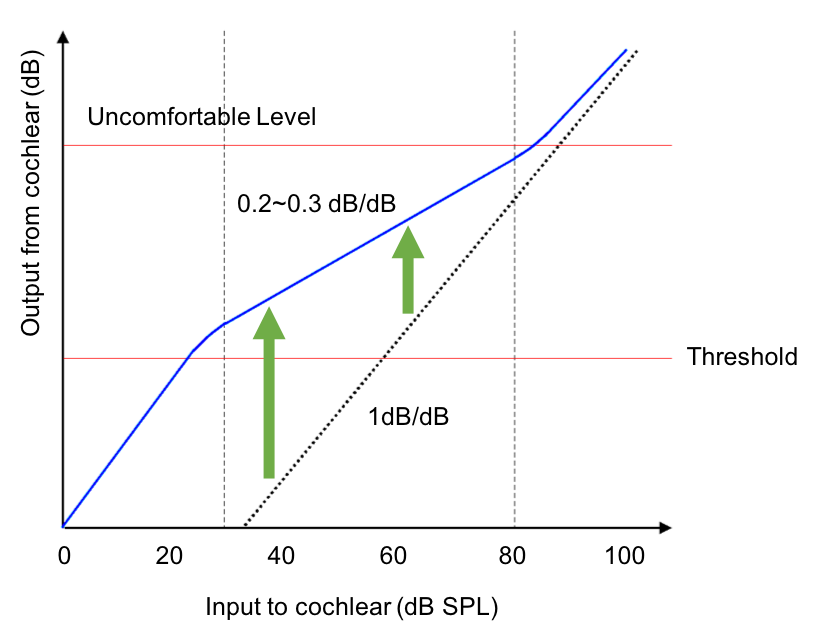
\includegraphics[width=8cm]{image/Hearin_Cmp.png}
%       \caption{圧縮特性を示す蝸牛入出力関数の概念図.横軸は蝸牛へ入力されるレベル, 縦軸は蝸牛から出力される内部レベル. 入力レベルが30~80dBの音圧レベルにおいて傾きが穏やかになり, 圧縮的である. 可聴域の音圧レベルの範囲を圧縮して内部表現上で表すことから圧縮特性と呼ばれる.}
%       \label{fig:Hear_Cmp}
%   \end{center}
% \end{figure}
%-----------------------------------------------------------------
\section{結果}
%-----------------------------------------------------------------

%-----------------------------------------------------------------
\subsection{危険度評価実験の結果}\label{danger_Rst}
%-----------------------------------------------------------------
図\ref{fig:danger_result}は交通音の危険度評価実験における加工条件や速度ごとの危険度評価の平均値を示している.
図\ref{fig:danger_result}から平均音圧が同じである場合, 健聴条件, 音圧低下条件, 模擬難聴条件の順に危険度が高いと判断されたことが分かる. 交通音の危険度評価における老人性難聴の影響を統計的に検討するために, 加工条件と音圧条件を要因とした有意水準5\%の二要因分散分析を行った. その結果, 加工条件について主効果が認められ[$F(2, 18) = 377.13$, $p<0.0001$], 音圧条件についても主効果が認められた[$F(1, 9) = 367.60$, $p<0.0001$]. さらに, 加工条件と音圧条件の交互作用が有意確率5\%で認められた[$F(2, 18) = 4.95$, $ p=0.0194$]. 加工条件と音圧条件との組み合わせ6種を要因としてShafferのMSRB(Modified Sequentially Rejective Bonferroni)法による検定を有意水準5\%で適用したところ, 全ての要因間に有意差が認められた.
%また, 速度(60, 100~km/h)と加工条件を要因として二要因分散分析($\alpha=0.05$)を行ったところ, 加工条件と速度条件の主効果が有意であった.
\par
次に, 車の走行速度による危険度評価への影響を検証するため, 車の走行速度が60, 100~km/hである刺激音の結果を抽出して解析を行った. 60, 100~km/hの速度を抽出した理由は, どちらも全体に占める標本数の割合が大きくかつ標本数にあまり差がない組み合わせであるためである(60~km/h N=1440, 100~km/h N=1200).速度, 加工条件, 音圧条件を要因とした有意水準5\%の三要因分散分析を実施したところ, それら全ての要因の主効果が有意であり[速度 : $F(1, 9) = 34.65$,  $p=0.0002$  加工条件 : $F(2, 18) = 77.33$, $p<0.0001$, 音圧条件 : $F(1, 9) = 446.80$, $p<0.0001$], 加工条件と音圧条件の交互作用が認められた[$F(2, 18) = 5.96$, $p=0.0103$].
%-----------------------------------------------------------------
\subsection{速度評価実験の結果}\label{Speed_Rst}
%-----------------------------------------------------------------
\par
図\ref{fig:speed_result}は交通音の速度に関する一対比較から得られた速度評価の分布図である. 健聴条件と模擬難聴条件において同じ元音源ごとの速度評価を比較すると, 全ての音源において模擬難聴条件のほうが健聴条件よりも遅く評価されたことが読み取れる. また, 健聴条件と模擬難聴条件の双方において, 60~km/hと100~km/hの音源の順序が入れ替わるようなことはなかった. さらに, 100~km/hの音源同士では加工条件ごとに比較するとどちらも同じ順序であるが, 60~km/hの音源同士を比較すると加工条件によって評価順序が異なっており, 模擬難聴条件のほうがその配置間隔も狭かった.



%模擬難聴条件の音源のほうが健聴条件よりも遅く知覚されていることが分かる.

% 加工条件と音圧条件を要因とした二要因分散分析($\alpha=0.05$)を行ったところ, 加工条件と音圧条件に主効果が認められた. さらに両条件間に交互作用が認められた.
% 図\ref{fig:danger_result}は交通音の危険度評価実験における加工条件や速度ごとの危険度評価の平均値を示している. 加工条件と音圧条件を要因とした二元配置の分散分析を行ったところ, 加工条件について主効果が認められ, 音圧条件についても主効果が認められた[$F(2, 3594) = 2449.340$, $p<0.0001$]. さらに, 加工条件と音圧の交互作用が有意確率5\%で認められた[$F(2, 3594) = 15.2010$, $ p<0.0001$]. また, 速度(60, 100km/h)と加工条件を要因として二元配置の分散分析を行ったところ, 加工条件の主効果が認められ[$F(2, 2634) = 1057.858$, $p<0.0001$], 速度要因間に有意差が見られた[$F(1, 2634) = 31.888$, $p<0.0001$]. 加工条件と速度の交互作用は見られなかった.
% 図\ref{fig:speed_result}は交通の危険度評価実験から得られた速度評価の分布図である. 図\ref{fig:speed_result}から, 模擬難聴条件の音源のほうが健聴条件よりも遅く知覚されていることが分かる.

% 図\ref{fig:danger_result}において, 加工条件間に有意差があったことから, 老人性難聴により交通音の危険性が低く評価されると推定される.
% 速度と加工条件の交互作用は見られなかったが, 60, 100km/hという大きな差がある音源にもかかわらず似た危険度として評価されたため, 速度感の一対比較を実施し詳細を調査した。
% 図\ref{fig:speed_result}からは, 模擬難聴条件が健聴条件よりも全体的に遅く評価されたことが読み取れる. 両加工条件で60, 100km/hの判断はつくようであるが,  60kmの音源に関しては並び順が異なっており、音源間の距離も狭い。老人性難聴により速度の知覚に多少の変化が生じている可能性を否定できない.

% 図\ref{fig:danger_result}は交通音の危険度評価実験における加工条件や速度ごとの危険度評価の平均値を示している. 加工条件と音圧条件を要因とした二要因分散分析(α=0.05)を行ったところ, 加工条件について主効果が認められ, 音圧条件についても主効果が認められた. さらに, 加工条件と音圧の交互作用が認められた. また, 速度(60, 100km/h)と加工条件を要因として二要因分散分析(α=0.05)を行ったところ, 加工条件の主効果が認められ, 速度要因間に有意差が見られた. 加工条件と速度の交互作用は見られなかった.
% 図\ref{fig:speed_result}は交通の危険度評価実験から得られた速度評価の分布図である. 図\ref{fig:speed_result}から, 模擬難聴条件の音源のほうが健聴条件よりも遅く知覚されていることが分かる.

%危険度評価実験の速度ごとの値
\begin{figure}[H]
  \begin{center}
      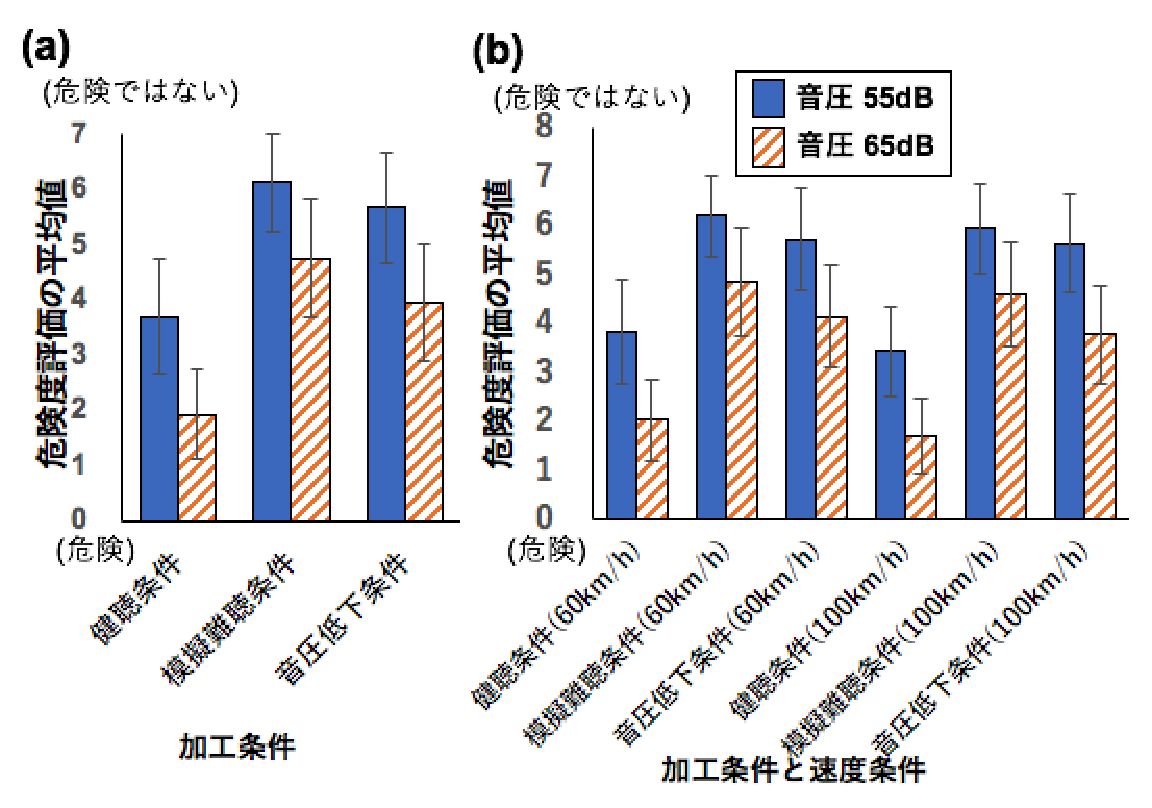
\includegraphics[width=8cm]{image/danger_result.eps}
      \caption{(a)加工条件(健聴条件, 模擬難聴条件, 音圧低下条件) + 音圧条件(55, 65~dB)における危険度評価の平均値と標準偏差, (b)速度(60, 100~km/h) +加工条件+音圧条件による危険度評価の平均値と標準偏差}
      \label{fig:danger_result}
  \end{center}
\end{figure}

\vspace{-12truemm}

%危険度評価実験の速度ごとの値
\begin{figure}[H]
  \begin{center}
      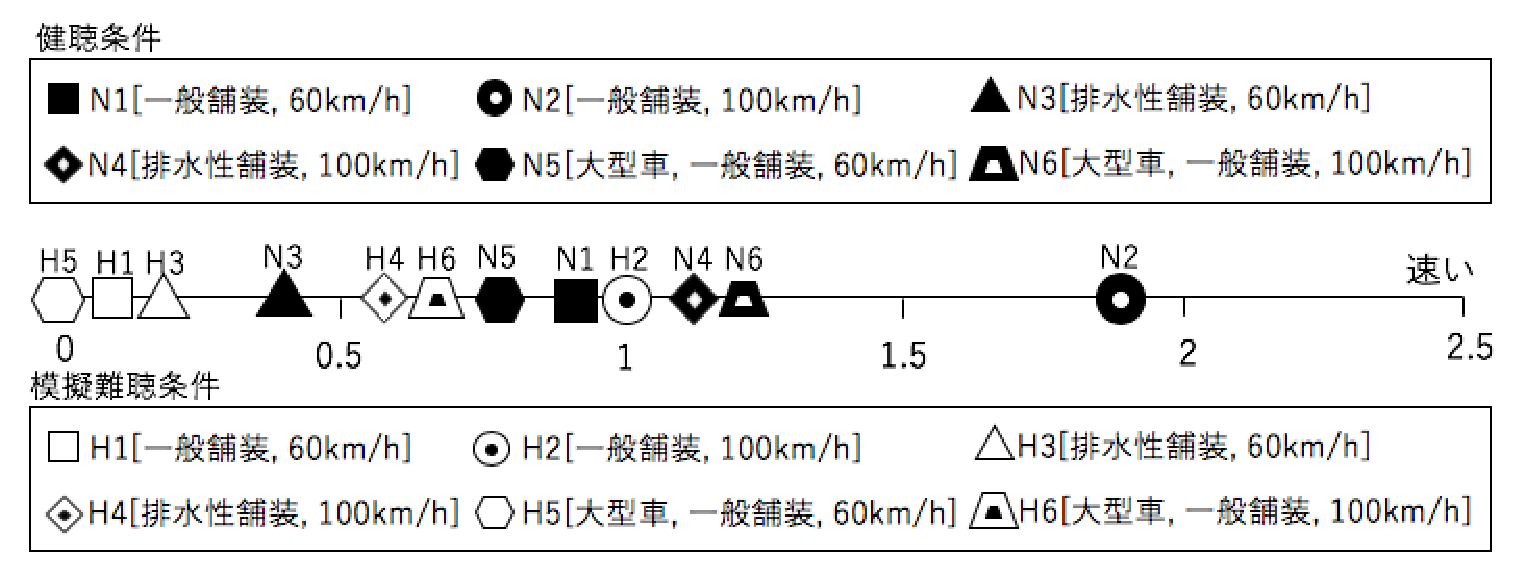
\includegraphics[width=8cm]{image/speed_result.eps}
      \caption{速度に関する一対比較の結果}
      \label{fig:speed_result}
  \end{center}
\end{figure}

\vspace{-8truemm}


%-----------------------------------------------------------------
\section{考察}
%-----------------------------------------------------------------

図\ref{fig:danger_result}において, 加工条件に主効果が認められたことから, 老人性難聴により交通音の危険性が低く評価されると推定される.
速度と加工条件の交互作用は見られなかったが, 60, 100~km/hという大きな差がある音源にもかかわらず似た危険度として評価されたため, 速度感の一対比較を実施し詳細を調査した.
図\ref{fig:speed_result}からは, 模擬難聴条件が健聴条件よりも全体的に遅く評価されたことが読み取れる. 両加工条件で60, 100~km/hの判断はつくようであるが,  60~km/hの音源に関しては並び順が異なっており, 音源間の距離も狭い. 老人性難聴により速度の知覚に多少の変化が生じている可能性がある.

% 図\ref{fig:danger_result}において, 健聴条件と模擬難聴条件の間に有意差があったことから, 老人性難聴により交通音の危険性が低く評価されると推定される.
% 速度と加工条件の交互作用は見られなかったが, 60, 100km/hという大きな差がある音源にもかかわらず同じ危険度であると評価されることもあったため, 速度を指標とした一対比較による検定を実施し, 速度判断についてより詳しく調査することとした.
% 図\ref{fig:speed_result}に示す速度評価の分布図からは, 模擬難聴条件が健聴条件よりも全体的に遅く評価されたことが読み取れる. 健聴条件においても模擬難聴条件においても60, 100km/hの判断はつくようであるが,  60kmの音源に関しては加工条件によって並び順が異なっている. したがって, 老人性難聴により速度の知覚に多少の変化が生じている可能性を否定できない.
% こういった知覚への影響が高齢者の交通事故における死亡率が高い要因の一つかもしれない.


%-----------------------------------------------------------------
\section{まとめ}
%-----------------------------------------------------------------

本研究では, 老人性難聴が交通音の危険性の知覚に与える影響について模擬難聴を用いて検討した. 老人性難聴によって交通音に対する危険性が健聴者よりも低く評価され, 速度判断についても変化が生じている可能性が示唆された.

%-----------------------------------------------------------------
\paragraph{謝辞}
%-----------------------------------------------------------------
 本研究の一部は、科研費16H01734, 18K10708およびJST日本‐台湾研究交流平成 30年度課題の支援を受けた.
 %本研究を進めるにあたり, 本学情報・知能工学系の松井准教授には主指導教員として丁寧かつ熱心なご指導を賜りました. 深く感謝申し上げます. また, 日常の議論を通じて多くの知識や示唆を頂戴いたしました聴覚心理物理学研究室の皆様に感謝の意を表します.

%-----------------------------------------------------------------
% 参考文献
%-----------------------------------------------------------------

\begin{thebibliography}{9} % 参考文献が10以上ある場合は{99}とする
\itemsep -5pt             % 項目の間隔微調整用
\bibitem{nagae2014hearing} Nagae, M., et al, APSIPA, 2014 Asia-Pacific, pp.1-4, 2014.
\bibitem{日本建築学会2004建築と環境のサウンドライブラリ} 日本建築学会, 建築と環境のサウンドライブラリsmile2004, 2004
\bibitem{iso1984acoustics} ISO7029, 2000
\end{thebibliography}

\end{document}
